%!TEX root = karulf-thesis.tex
\chapter{Human-Robot Interaction}
\label{chapter:ui}

Human-Computer Interaction, HCI, is the study of how humans interface with technology. This includes traditional interfaces, like graphical user interfaces controlled with a mouse and keyboard, as well as alternative interfaces such as the accelerometers in the Nintendo Wii™ controller or the motion tracking system in the Microsoft Kinect™.

Despite the advances in efficacy and popularity of non-traditional devices, the remainder of this paper will be limited to devices standard on most computer systems, e.g., a monitor, mouse, and keyboard. In Section~\ref{section:futurework} I will briefly introduce where alternative interfaces would enhance the proposed interface.

\section{Robotic User Interfaces}
% From wds@

Human-Robot Interaction is a subset of Human-Computer Interaction which focuses on how humans interface with robots. In his survey paper on HRI, Dr. Michael Goodrich introduces five attributes, shown in Figure~\ref{fig:five-attributes} that define the interactions between humans and robots (Goodrich 216-217).

\begin{figure}[ht]
	\makebox[\textwidth]{\hrulefill}
	\begin{list}{$\bullet$}
		\item Level of behavior and autonomy
		\item Nature of information exchange
		\item Structure of the team
		\item Adaptation, learning, and training of people and the robot
		\item Shape of the task
	\end{list}
	\makebox[\textwidth]{\hrulefill}
	\caption{Five attributes of Human-Robot Interaction \label{fig:five-attributes}}
\end{figure}

In the world of robotics, autonomy is defined as the extent of actions a robot may take independently. One of the core ideas behind RIDE is the idea that autonomy may vary depending on context. In the Section~\ref{section:autonomy} I will introduce the idea of ``sliding autonomy'' and how we implement it within the RIDE interface.

Information exchange simply describes the data that flows between a robot and a human. This description characterizes the amount of data that is passed and how the information is visualized. Much like with autonomy, I propose an interface that adapts the nature of information exchange based on context. In Section~\ref{section:infoexchage} I will introduce our refinements to the existing work in this field.

% TODO: Paragraph on Structure of the team

\subsection{Autonomy}

Autonomy, independent robot behavior, is an important factor in HRI design. The relationship between a robot and a human, as provided through the interface, can be viewed or conceptualized along the lines of a continuum or a scale of autonomy. Teleoperation represents one end of the spectrum, where the robot exhibits no qualities of autonomous behavior. On the other hand, a fully autonomous robot, that ignores human input, represents the other extreme of autonomy. A simple scale of autonomy can be found in Figure~\ref{fig:autonomy}. \cite{Goodrich_Survey}


\begin{figure}[ht]
\begin{center}
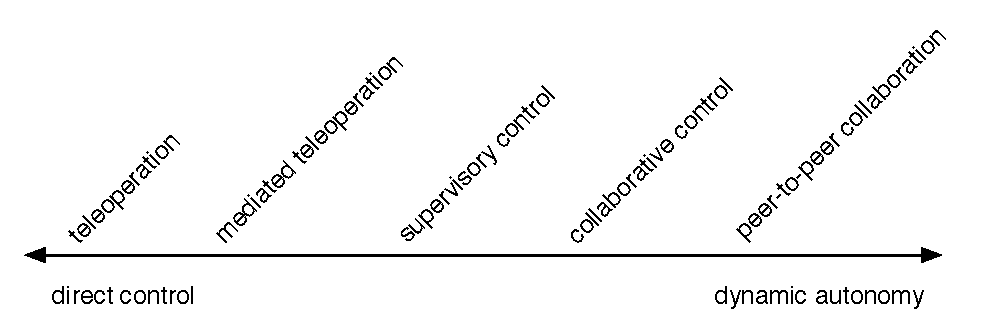
\includegraphics[width=5in]{images/autonomy.pdf}
\caption{Scale of Robot Autonomy\label{fig:autonomy}}
\end{center}
\end{figure}

% Awk. -ek
Robots, as they presently exist, have a fairly limited set of autonomous actions available. As a result, most interfaces, currently, are artificially conservative in their autonomy due to limitations in artificial intelligence. As research into artificial intelligence and machine learning grows, a much more diverse set of autonomous behaviors will inevitably become available. As user interface designers, we are tasked to create extensible interfaces to support future behaviors.

The Robot Interactive Display Environment, also known as RIDE, employs a dynamic approach known as sliding autonomy. This allows the human and the robot to change the level of autonomy as needed. RIDE allows the human to increase or decrease the level of autonomy on a per robot basis. In contrast, the robots are capable of only decreasing the level of autonomy. For illustration purposes, consider a robot that explores a warehouse. If the robot planned a poor navigation path, a user could manually specify the waypoints of an optimal path. If the robot is unable to complete the specified path due to an obstruction in the path, the robot could ask the user to directly teleoperate around the obstacle. Once free of the obstruction, the user would input a new set of goal coordinates and allow the autonomous navigation system to resume control.

% Needs tightening -ek
While the RIDE application does not specify any restrictions, I have elected to restrict the scope of my thesis to allow for a more careful examination of environmental searching within the range of supervised autonomy. In Section~\ref{section:futurework} I explain how these principles of RIDE could be adapted to support more autonomous behavior.

\subsection{Information Exchange}
\label{sub:info_exchange}
The nature of information exchange defines the flow of data between the human and the robot. What information is provided, how it is represented, and when it is communicated are all properties of the interface design. This encompasses low-level communication of navigation and sensor data as well as high-level commands sent from the human. 

The purpose of visualization interfaces is to represent the one-way exchange of information from the robot to humans. This data typically includes location information, laser or sonar readings, battery readings, accelerometer readings, and map data. Original interfaces were written to be accessible programatically. These interfaces were slowly adapted to display sensor data graphically, but the resulting interfaces were disjoint and required operator training. Examples of these 2D user interfaces can be seen in Figure~\ref{existing-robot-ui}.

In 2007 Dr. Curtis Nielsen introduced an ecological user interface with the goal of combining sensor data into a single, integrated display. Nielsen designed his interface to for effective teleoperation, the technique of controlling a robot remotely. In his study, Nielsen compared an integrated 3D user interface to a simple 2D user interface for several environment searching tasks. The 3D user interface displayed combined sensor data through a single viewport while the 2D user interface displayed the same data through individually. The study found the 3D interface decreased collisions and decreased task completion time. \cite{Nielsen_Teleoperation}

Nielsen attributes the success of the 3D interface to improved situational awareness. The observed effect of situational awareness and context on interface effectiveness is congruous with the findings of other researchers. \cite{Nielsen_Teleoperation}

A limitation of Nielsen's interface is that it's focus on teleoperation leaves the robot without autonomy. While teleoperation may be optimal for single robot environments it does not allow for concurrent robot control. This limitation requires an human operator for every active robot.
